\section{Introduction}
The market for personal electric transport is a burgeoning space with significant innovation and financial backing. 
\textit{Boosted Boards}, makers of an electric longboard product, raised US\$467,000 in crowdfunding on Kickstarter \cite{boostedkickstart} before collecting another US\$326,000 in series A funding during the early phases of development \cite{boostedfunding}. 
Similarly, \textit{OneWheel} raised US\$630,000 on Kickstarter \cite{onewheelkickstart} and an additional US\$3.2 million in series A funding \cite{onewheelfunding} for their self stabilizing monowheel device. 
This combination of significant public interest via Kickstarter and an outpouring of funding from venture capitalists for what were still early stage transportation products demonstrates significant need for solutions in this space.
Mathematical modeling techniques and considerations for these types of systems are explored in detail in this report.
\subsection{Context \& Motivation}
To provide sufficient background for the broader design problem being addressed, some analysis of the present state of commuting and urban centers is provided, followed by a brief outline of the system selected for demonstrating the chosen modeling techniques.
\subsubsection{Changing Cities}
By 2050, it is projected that 86\% of the developed world will reside in urban areas \cite{Economist}. 
As a result of the adoption of the motorized vehicle, cities have become increasingly multi-centred, with retail parks and industrial estates far removed from city centers \cite{SustainableTransport}. 
This evolving, sprawling nature of modern cities renders traditional public transport largely ineffective at efficiently transporting the population within cities \cite{SustainableTransport}. 
A British study showed that 83\% of commuting trips and 90\% of business trips in that country involved only a single passenger in a car \cite{NTS}, highlighting that the supply of mass, group transit does not meet the travel demands of modern society.

The lack of effective transportation infrastructure also has a considerable impact on the environment. 
The United States Environmental Protection Agency has determined that 14\% of global emissions are as a result of the transportation sector \cite{EPA}. 
Meanwhile, a Belgian case study showed that 47\% of trips and 54\% of distance traveled in that country was for the purpose of urban commuting \cite{Belgium}. 
Clearly, the environmental impact of urban transportation is considerable.

Research has also concluded that an effective transportation system for a modern city must \cite{SustainableTransport}:

\begin{enumerate}
	\item Be available on demand
	\item Go non-stop from start to destination
	\item Be easily accessible and offers a full choice of destinations
	\item Be strongly environmentally friendly
	\item Be low cost
	\item Integrate well with other forms of transport
	\item Have demonstrably high safety together with personal security
\end{enumerate}

Personal electric transport has the potential to satisfy the transportation demands of a modern city. 
This type of transportation mechanism is user operated, meaning it is indeed available on demand and is accessible. 
Additionally, it is inherently portable and thus integrates well with other forms of transport. 
Using an appropriate power source will ensure that the transportation device can travel non-stop to and from a multitude of destinations at a low cost, while a well designed stabilizing mechanism can ensure personal safety. 
To further develop these concepts, with particular focus on developing stabilizing control systems for personal transport, the RipStik is used as a representative example.

\subsubsection{The RipStik}

A caster board, known commercially as a RipStik, is a two-wheeled, human powered vehicle. 
The board is similar to a skateboard; however, it features two independent platforms, separated by a central torsion spring.
An inclined free spinning caster is attached to each platform. 
This design gives the caster board rider the unique ability to generate propulsion without removing their feet from the board through a series of small turns. 
This configuration also allows for tighter turning and more responsive speed control when compared to a skateboard. 

\begin{figure}[!htb]
	\centering
	\minipage{0.5\textwidth}
	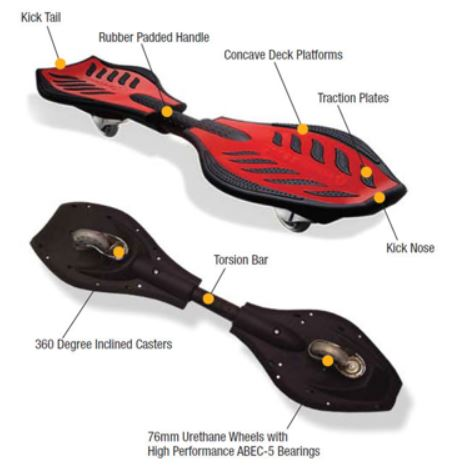
\includegraphics[width=\linewidth]{RipStik.JPG}
	\caption{Detailed description of the components of a RipStik \cite{PIC}}\label{fig:RipStik}
	\endminipage
\end{figure}
\par
The RipStik presents an interesting research opportunity because the associated motions and physics are unintuitive.
As a result, comprehensive testing and design metrics are required as there are no implicit assumptions to be made about the device's operation. 
This allows the technology developed in modeling and controlling the RipStik to be applied to a large variety of systems. 
Furthermore, many of the core concepts like wheel motion and stability are highly applicable in the domain of electric transportation. 

The design of a control system for a personal transportation device needs to be done with careful consideration for a number of external factors. 
Aside from the challenges associated with the development of the mathematical model and control system, issues pertaining to the patents for transport systems \cite{casterboardPatent} and restricted operation of certain devices \cite{TOLaws} may represent a barrier in bringing theses products to market. 
Additionally, a mechanical system will be required to execute the commands of the control system. 
The difficulties associated with the recycling of batteries \cite{BatteryRecharge}, housing \cite{PlasticAssessment} and motors may threaten the environmental feasibility of the final design. 
The system may also be susceptible to ``hacking'' by outside sources \cite{DEFCON}, which could pose a significant safety risk to the operator. 
These issues will be analyzed to mitigate the associated risks and properly weigh relevant environmental, social and economic trade-offs.
This area of study has the potential to redefine urban commuting across the world by introducing a safe, cost-effective and environmentally-friendly option for short distance travel. 

\subsection{Problem Definition}

Aside from select innovative exceptions, current methods of electric personal transport are limited in both mechanics and utility by an adherence to more traditional form factors such as the skateboard and bicycle. 
As an example of an alternate transportation system, a full control law for a RipStik will be developed and tested. 
The development of this control law will first require a complete, working mathematical model of the RipStik and a custom tool to visualize the model and control law outputs on a 3D model of the device. 
Simplifications and assumptions will need to be made in order to develop a working model of the system. 
These simplifications and assumptions will be carefully scrutinized to ensure that they do not compromise the ability of the model to be applied to other complex mechanical systems. 
A control system will then be developed to propel the RipStik with consideration to triple bottom line implications, including minimizing power requirements and ensuring operator safety. 
Trade-offs will be made in the development of the control system to find the system which best addresses the problem constraints and social, economic and environmental considerations. 

\subsection{Technical Background}
To develop a comprehensive mathematical model and stabilizing control law for a system as complex as the RipStik, a number of mathematical tools are necessary.

\subsubsection{Euler Angles}

Euler angles describe the orientation of a body in an inertial reference frame.
These orientations are represented by rotations of three angles: yaw ($\theta$), pitch ($\psi$), and roll ($\alpha$).
With the Euler angles defined, rotation matrices can then be created for the bodies of a system.

These rotation matrices are defined by \cite{Lewis}:

\begin{equation}
\label{eq:RotM}
R =
\begin{bmatrix} 
\cos\alpha\cos\psi & \cos\alpha\sin\psi\sin\theta - \cos\theta\sin\alpha &\cos\alpha\cos\theta\sin\psi+\sin\alpha\sin\theta\\
\cos\psi\sin\alpha & \cos\alpha\cos\theta+\sin\alpha\sin\psi\sin\theta & \cos\theta\sin\alpha\sin\psi - \cos\alpha\sin\theta\\
-\sin\psi & \cos\psi\sin\theta & \cos\psi\cos\theta 
\end{bmatrix}.
\end{equation}

The rotation matrix R can be used to describe a rotation from a body-fixed frame to the inertial frame \cite{VTOL}.

\subsubsection{Lagrangian Mechanics}

Lagrangian mechanics can be used in place of Newtonian mechanics when trying to accurately model highly complex systems.
In these elaborate systems, constraint forces can be implemented to eliminate degrees of freedom and reduce the complexity of the system \cite{LagrangeEquations}. 
Additionally, Lagrangian equations are invariant to changes of coordinate systems \cite{LagrangePowerpoint}.

The Lagrangian function is represented by $L$, and is defined as the difference between kinetic and potential energies in a system modeled using positions and velocities \cite{NonholonomicPowerpoint}.
In the equation, $T$ represents the kinetic energy and $V$ represents the potential energy.
The mathematical formulation for the Lagrangian is given by

\begin{equation}
\label{eq:Lagrange}
L = T - V.
\end{equation}

\subsubsection{Euler-Lagrange Equation}

In Lagrangian mechanics, the equations of motion are given by the solutions to a second order partial differential equation known as the Euler-Lagrange equation \cite{Lewis}. 
For this purpose, the Euler-Lagrange equation is given by:

\begin{equation}
\label{eq:EL}
\frac{\text{d}}{\text{dt}} \bigg(\frac{\partial \text{L}}{\partial \dot{\text{q}}_{i}}\bigg) - \frac{\partial \text{L}}{\partial \text{q}_{i}} = 0.
\end{equation}
The Euler-Lagrange equations are equivalent to Newton's second law \cite{NonholonomicPowerpoint}, and are implicit second-order differential equations applied to a given coordinate system \cite{Lewis}.
\par
The unconstrained equations of motion encompass each degree of freedom in the system, and are of the form:

\begin{equation}
\label{eq:UEOM}
G_{jk} \ddot{q}^k + \Gamma_{jkl} \dot{q}^k\dot{q}^l  = F_{j}.
\end{equation}

In Equation \ref{eq:UEOM}, $G_{jk}$ represents the acceleration coefficients of the system, $\Gamma_{jk}$ represents the velocity coefficients of the system, and $F_j$ represents the potential forces in the system.

\subsubsection{Nonholonomic Constraints}

Nonholonomic constraints are implemented to restrict velocities in a system \cite{LagrangeEquations}.
Lagrange multipliers are added to the unconstrained equations of motion to represent unknown constraint forces \cite{ClassicalMechanics}.
\par
The forces can then be determined from the system of equations:

\begin{equation}
\label{eq:CFE}
G_{jk} \ddot{q}^k + \Gamma_{jkl} \dot{q}^k\dot{q}^l  = \lambda_{a}\omega_{j}^{a} + F_{j}
\end{equation}
and
\begin{equation}
\label{eq:CV}
\omega_{j}^{a} \dot{q}^{j} = 0.
\end{equation}

Equation \ref{eq:CFE} is identical to the unconstrained equations of motion with the added $\lambda_{a}$ term, representing the constraint forces.
Equation \ref{eq:CV} represents the velocity constraints. 
\par
When solving for the constraint forces, the system is a Differential Algebraic Equation (DAE).

\subsubsection{Linear Quadratic Regulator Control}
The linear quadratic regulator (LQR) algorithm is a method in control theory used to technique used to determine the optimal control gains for a state feedback controller for a linear system with a quadratic cost function \cite{LabManual}.

For the purpose of this project, linear control systems $\Sigma$ of the form
\begin{equation}
\dot{x}(t) = Ax(t) + Bu(t)
\end{equation}
where $A \in \R^{m \times m}$ and $B \in \R^{m \times l}$ are considered.
The associated quadratic cost function for time interval $[t_{0},t_{1}]$ is then 
\begin{equation}
\eta(u) = \int_{t_{0}}^{t_{1}}x^{T}(t)Qx(t)+u^{T}(t)u(t)dt
\end{equation}
where $Q \in \R^{m \times m}$ is the state weighting matrix associated with the degrees of freedom and their derivatives $(q, \dot{q})$ in the system. Note that no weightings are associated with the control inputs at this stage, though they may be necessary when considering the broader design impacts (see section \ref{sec:Tradeoff}. Tuning the cost function weighting matrix $Q$ allows emphasis to be placed on stabilization of certain degrees of freedom to better meet design goals for the particular application.

The optimal control gains $K$ are then computed from
\begin{equation}
K = B^{T}X_{r}
\end{equation}
where  $X_{r}$ is the solution to the continuous algebraic Riccati equation \cite{RicattiSolve}.
\begin{equation}
A^{T}X_{r} + X_{r}A - (X_{r}B)(B^{T}X_{r}) + Q = 0.
\end{equation}

\subsection{Literature Review}
\subsubsection{A Nonlinear Mathematical Model for a Bicycle}
To gain a clearer perspective of the overall procedure and concepts involved in modeling a complex mechanical system of this nature, a number of similar mathematical models for other modes of personal transportation were analyzed.
In particular, \textit{A Nonlinear Mathematical Model for a Bicycle} \cite{BikeModel} provides a clear example of establishing the necessary coordinate systems and transformation matrices associated with the interconnections and internal angles within the bicycle.
This model includes the rolling dynamics of the wheels and discusses the minutiae of elements like the wheel crown radius, demonstrating the complexity they add to the model before removing these elements to provide a more manageable model.
The final model is also constructed under the assumption that the rider remains stable and upright, allowing the roll angle of the bicycle to be linearized, further facilitating interpretation of the final modeling results. 
%%%%%%%%%%%%%%%%%%%%%%%%%%%%%%%%
%%%%SHOULD WE INCLUDE AN IMAGE
%%%%Is wheel crown radius not self explanatory
%%%%%%%%%%%%%%%%%%%%%%%%%%%%%%%%

\subsubsection{Modeling and Control of Casterboard Robot}
In the paper \textit{Modeling and Control of Casterboard Robot} \cite{CasterboardRobot}, Kinugasa et al. discuss similar concepts and their application in the context of a casterboard, however, the overarching goals and product were distinct from the defined problem.
The group from Osaka University developed a highly simplified model, omitting the problem of stability and simplifying the dynamics of the caster rotation using a holonomic constraint. 
They then used this to develop a locomotion control method for the casterboard before implementing, testing and tuning it on a physical robot constructed to match the geometry of the casterboard.

%%%%%%%%%%%%%%%%%%%%%%%%%%%%%%%%
%%%%SHOULD WE INCLUDE AN IMAGE
%%%%%%%%%%%%%%%%%%%%%%%%%%%%%%%%

